\documentclass[a4paper]{article}

\usepackage[english]{babel}
\usepackage[utf8]{inputenc}
\usepackage{amsmath}
\usepackage{graphicx}
\usepackage[colorinlistoftodos]{todonotes}

\title{CS5011 Machine Learning Contest Report}

\author{Rishiraj Surti, EE12B120\\
	author2\\
	author3\\}

\date{\today}

\begin{document}
\maketitle

\section{Sklearn SVM and Neural Network}

\section{LDA, QDA, KNN}

\section{LibSVM, Bayes, Adaboost}
\subsection{LibSVM}

\begin{table}
\centering
\begin{tabular}{l|l|l}
Algorithm & Source File & Output file \\\hline
SVM & svm\_rs.py & svm\_rs\_output\_*.py \\

\end{tabular}
\caption{\label{tab:widgets}List of files}
\end{table}




\begin{figure}
\centering
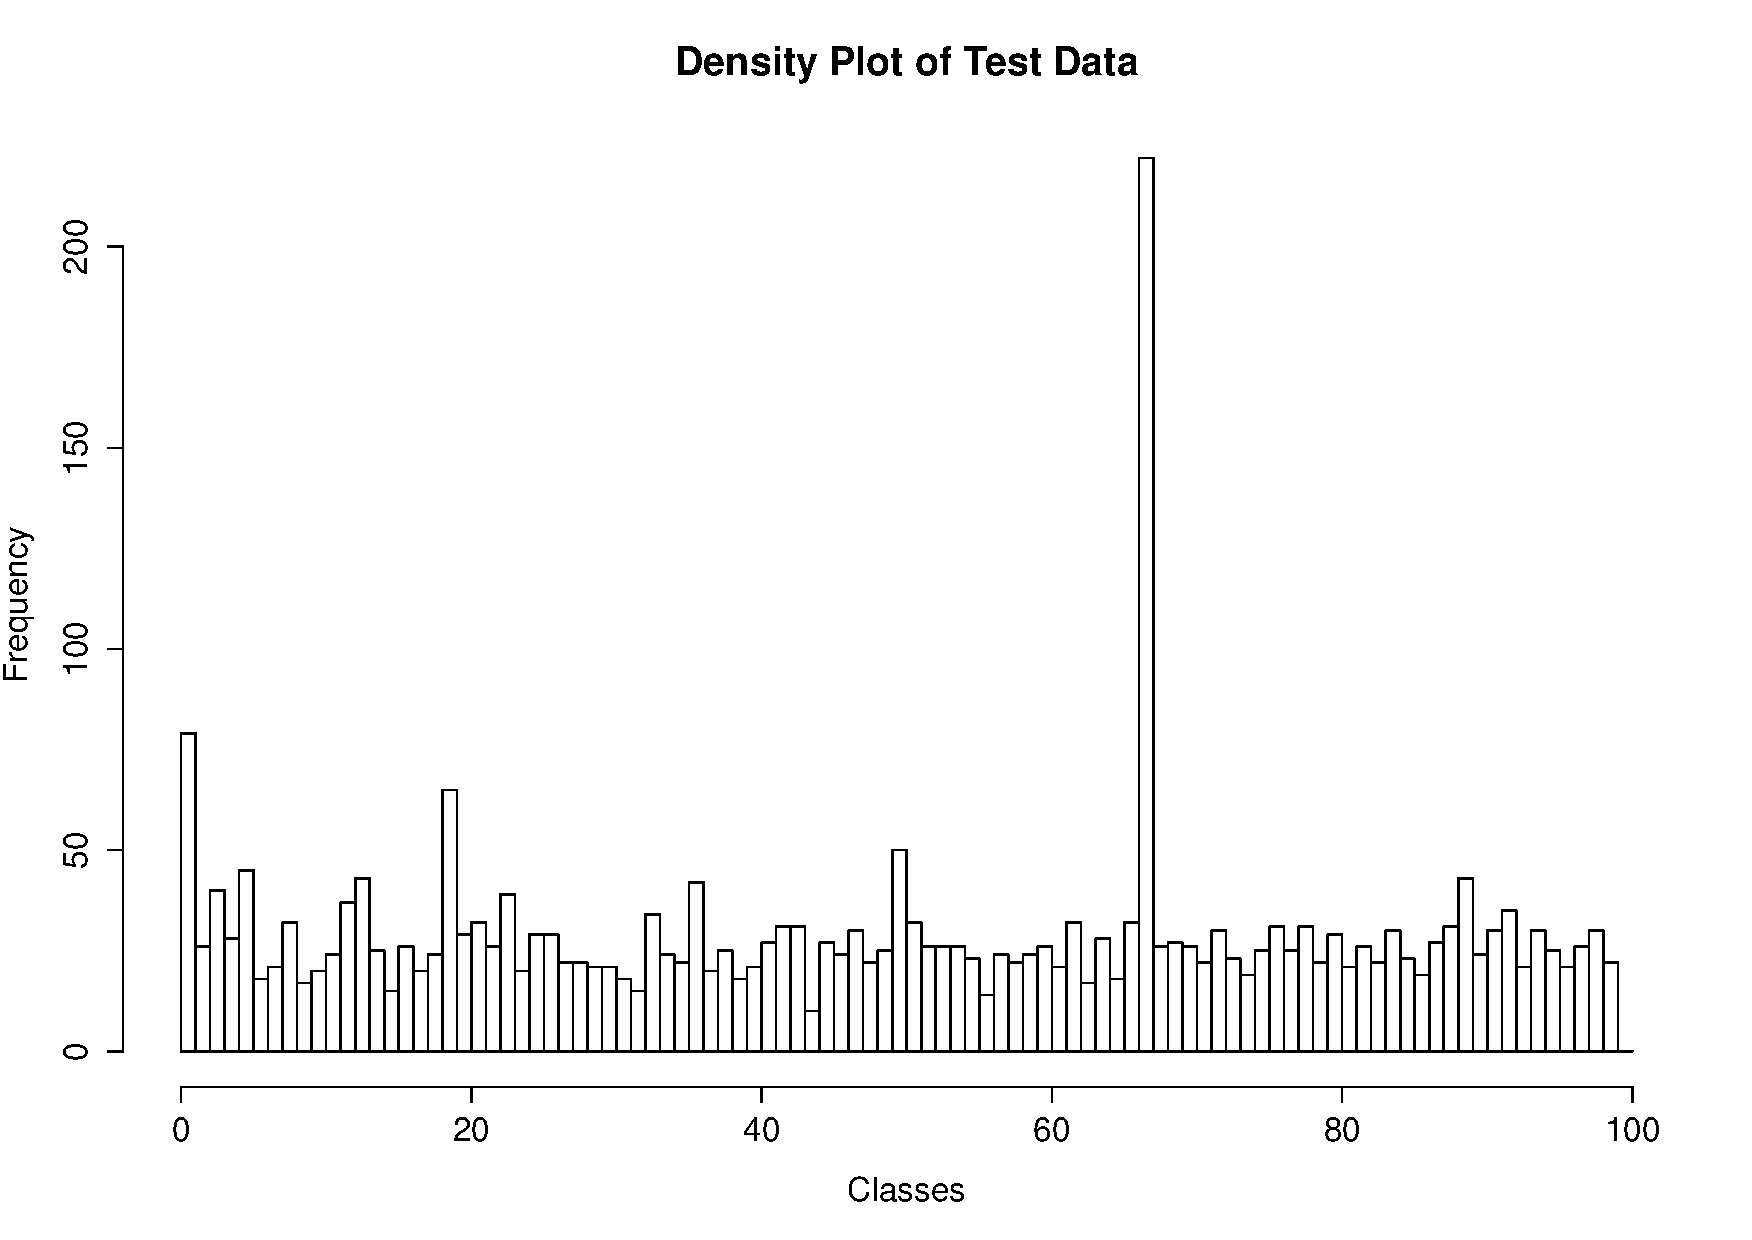
\includegraphics[width=1\textwidth]{../plots/TestData_targets.pdf}
\caption{\label{fig:data}Raw (unprocessed) data. Replace this figure with the one you've made, that shows the resistivity.}
\end{figure}

\begin{table}
\centering
\begin{tabular}{l|r}
Item & Quantity \\\hline
Widgets & 42 \\
Gadgets & 13
\end{tabular}
\caption{\label{tab:widgets}An example table.}
\end{table}


\begin{enumerate}
\item Like this,
\item and like this.
\end{enumerate}
\dots or bullet points \dots
\begin{itemize}
\item Like this,
\item and like this.
\end{itemize}
\dots or with words and descriptions \dots
\begin{description}
\item[Word] Definition
\item[Concept] Explanation
\item[Idea] Text
\end{description}

\end{document}
              